\section{Descripción TAMA}

\section{Selección de Ventana}

En \ref{KOU2009} se menciona una elección de \emph{frame step} y \emph{frame length} de 10s y 20s respectivamente. En el caso de nuestro corpus, quisimos buscar los parámetros que mejor se ajustaban a éste, manteniendo la superposición del 50\% entre ventanas sucesivas. Con lo que nos queda que $FL = 2 * FS$

¿Qué queremos optimizar? La métrica que elegimos para ésto es encontrar un balance entre un frame no tan grande (para no suavizar en exceso la curva) y que nos reduzca considerablemente la cantidad de indefiniciones; es decir, aquellas ventanas que tomamos en un interlocutor que no tienen ninguna interacción de su parte. Para ver ésto, graficamos la cantidad de indefiniciones en función del step tomado.

\begin{figure}
\centering
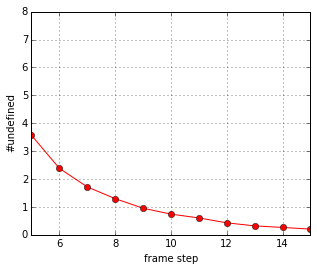
\includegraphics[width=10cm]{images/window_selection.png}
\end{figure}



Dentro del rango de $FS \in \{5'',6'', \ldots ,15'' \}$, graficamos para cada sesión, tarea y cada interlocutor las curvas de indefiniciones. A su vez, para mayor claridad, graficamos una curva que promedie todas las tareas de una sesión.


Para tener una visión general de lo que ocurría en todas las sesiones, graficamos una curva promedio de todas las sesiones. En ésta puede observarse que hasta $8''-10''$ hay un fuerte descenso de las indefiniciones, que luego se atenúa. Dado que en general tenemos tareas cortas, preferimos tomar $8''$ como step, y $16''$ como largo de ventana.

OBS: podríamos cambiar ésto a un boxplot!

\begin{figure}
\centering
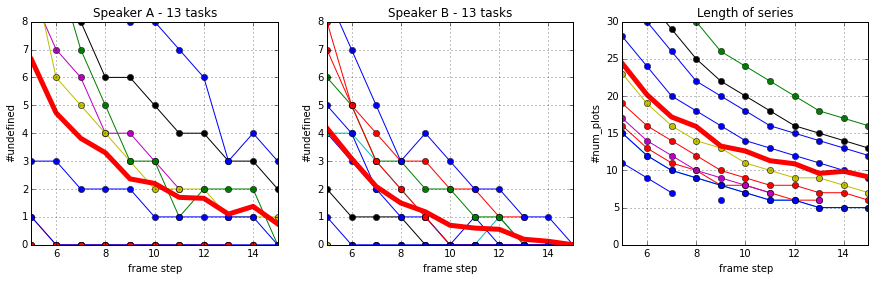
\includegraphics[height=5cm]{images/window_selection_for_session.png}
\end{figure}
